%%
%% This is file `cimsmple.tex',
%% generated with the docstrip utility.
%%
%% The original source files were:
%%
%% cimento.dtx  (with options: `sample')
%% 
%% IMPORTANT NOTICE:
%% 
%% For the copyright see the source file.
%% 
%% Any modified versions of this file must be renamed
%% with new filenames distinct from cimsmple.tex.
%% 
%% For distribution of the original source see the terms
%% for copying and modification in the file cimento.dtx.
%% 
%% This generated file may be distributed as long as the
%% original source files, as listed above, are part of the
%% same distribution. (The sources need not necessarily be
%% in the same archive or directory.)
%%%%%%%%%%%%%%%%%%%%%%%%%%%%%%%%%%%%%%%%%%%%%%%%%%
%%%%%%%%%%%%%%%%%%%%%%%%%%%%%%%%%%%%%%%%%%%%%%%%%%
%%%%%%%%%%%%%%%%%%%%%%%%%%%%%%%%%%%%%%%%%%%%%%%%%%
\ProvidesFile{cimsmple.tex}
      [1999/12/01 v1.4c Il Nuovo Cimento]
\documentclass{cimento}
\usepackage{multirow}
\usepackage{epsfig}


%%% MY DEFINITIONS

\providecommand{\MT}{\ensuremath{M_{\mathrm{T}}\xspace}}

\newcommand{\mH}{\ensuremath{m_{\mathrm{H}}}\xspace}
\newcommand{\MW}{\ensuremath{m_{\mathrm{W}}}\xspace}

\NeedsTeXFormat{LaTeX2e}
\RequirePackage{heppennames2}
\RequirePackage{xspace}
\RequirePackage{amsmath}

\newcommand{\MH}{\ensuremath{M_{\PH}}}
\newcommand{\fbinv} {\mbox{\ensuremath{\,\text{fb}^\text{$-$1}}}\xspace}
\newcommand{\GeV}{\ensuremath{\,\text{Ge\hspace{-.08em}V}}\xspace}
\newcommand{\gev}{\GeV}


\newcommand{\Pgg}{\PGg}
\newcommand{\Pgt}{\PGt}
\newcommand{\cPZ}{\PZ} % plain Z (no superscript 0)
\newcommand{\cPq}{\PQq} % generic quark

\newcommand{\cPqb}{\PQb} % b for b quark
\newcommand{\ET}{\ensuremath{E_{\mathrm{T}}}\xspace}
\newcommand{\et}{\ensuremath{E_{\mathrm{T}}}\xspace}
\newcommand{\PT}{\ensuremath{p_{\mathrm{T}}}\xspace}
\newcommand{\pt}{\ensuremath{p_{\mathrm{T}}}\xspace}

\newcommand{\ETm}{\ensuremath{E_{\mathrm{T}}^{\text{miss}}}\xspace}
\newcommand{\MET}{\ETm}





\title{Searches for the Standard Model Higgs Boson at CMS}

\author{Emanuele Di Marco for the CMS Collaboration}

\begin{document}

\maketitle

\begin{abstract}
We searched for the standard model Higgs boson using approximately
5 \fbinv of 7 TeV pp collisions data collected with the CMS detector
at LHC. We exclude at 95\% confidence level a standard model Higgs
boson with mass between 127.5 and 600 GeV. The expected 95\%
confidence level exclusion if the Higgs boson is not present is from
114.5 and 543 GeV. The most significant excess is observed at 125 GeV
with a local significance of $2.8 \sigma$. The excess is consistent
both with background fluctuation and a standard model Higgs boson with
mass of about 125 GeV.
\end{abstract}

%%%%%%%%%%%%%%%%%
%
% Introduction
%
%%%%%%%%%%%%%%%%%

\section{Introduction}

The scalar boson of the Brout-Englert-Higgs mechanism is the only
block of the standard model (SM)~\cite{SM1,SM2,Higgs1,Higgs2} whose
existence has not been verified experimentally. Therefore its search
is one of the most important aspects of the LHC program.
The Higgs boson has been ruled out at 95\% confidence level (CL) at
LEP~\cite{leplimits} with mass smaller than 114.4 GeV and at
Tevatron~\cite{tevatronlimits} with a mass in
the vicinity of 160 GeV .  Indirect constraints from precision
electroweak measurements favour a low mass Higgs
boson above the LEP limit and give the upper limit
%%%: $\MH<169$ GeV at 95\% CL from the standard fit and 
$\MH<143$ GeV at 95\% CL, including direct searches before LHC.
The dominant production mode at LHC is the gluon-gluon fusion followed
by the vector boson fusion (VBF) and associated production with a
vector boson (VH), each of which contributes less than 10\% of the
total production cross section. The decay branching ratios of the
Higgs boson vary with its mass and are dominated by bb and $\tau\tau$
at low mass and by WW and ZZ above 135 GeV.  The values of cross
section and branching ratios used in the following are taken from the
LHC cross section working
group~\cite{Dittmaier:2012vm}.
In 2011 CMS collected approximately 5 \fbinv of LHC data that are good
for all analyses.  The CMS detector is a multipurpose detector and is
extensively described in~\cite{CMSdetector}.The SM scalar boson search
is carried out in the mass range from 110 and 600 GeV.  The search
channels, as well as their optimization vary as function of the Higgs
mass.  The sensitivity of the different channels varies as function of
the Higgs boson mass.  The most sensitive channel at low mass, below
approximately 130 GeV, is the $\gamma\gamma$ channel. Between 130 and
200 GeV the WW channel is most sensitive, and above 200 GeV the
various ZZ channels take over.
%% \begin{table}[htbp]
%% \begin{center}
%% \small
%%   \caption[ ] {The 11 Higgs boson search channels. The most relevant information is indicated for each of the analyses.
%%   }
%%   \label{tab:channelsnew}
%% \begin{tabular}{ l c c c c}
%% \hline %-----------------------------------------------------------------------------------------------------
%% \hline %-----------------------------------------------------------------------------------------------------
%% \multirow{2}{*} {Channel}                            & $m_H$ range      & Luminosity     & Sub-      & $\mH$       \\
%%                                                      & (\GeV)           & (fb$^{-1}$)    & channels  & resolution           \\
%% \hline %-----------------------------------------------------------------------------------------------------
%%  {$\PH \to \Pgg\Pgg$                                     } & 110--150      & 4.8         &  2        & 1--2\%           \\
%%     $\PH \to \Pgt\Pgt \to e\tau_{\mathrm{h}}/\mu\tau_{\mathrm{h}}/e\mu+X$  & 110--145      & 4.6         &  9        & 20\%            \\
%%  $\PH \to \Pgt\Pgt \to \mu\mu+X$                                        & 110--140      & 4.5         &  3        & 20\%                  \\
%%  $W\PH \to e\mu \tau_h / \mu\mu \tau_h + \nu$'s                         & 100--140      & 4.7         &  2        & 20\%                   \\
%%     $(\PW/\cPZ)\PH \to (\ell\nu/\ell\ell/\nu\nu)(\cPqb\cPqb)$         & 110--135      & 4.7         &  5        & 10\%          \\
%%     {$\PH \to \PW\PW^* \to 2\ell 2\nu$                      } & 110--600      & 4.6         &  5        & 20\%           \\
%%  $W\PH \to \PW(\PW\PW^*) \to 3\ell 3\nu$                                & 110--200      & 4.6         &  1        & 20\%              \\
%%     {$\PH \to \cPZ\cPZ^{(*)} \to 4\ell$                      } & 110--600      & 4.7         &  3        & 1--2\%         \\
%%     $\PH \to \cPZ\cPZ^{(*)} \to 2\ell 2q$  & $\left\{ \begin{array} {l} \textrm{130--164} \\ \textrm{200--600} \end{array} \right. $  & 4.6  &  6     & $ \begin{array}{l}  3\% \\ 3\% \end{array}$ \\
%%     $\PH\to\cPZ\cPZ \to 2\ell 2\tau$                                       & 190--600      & 4.7         &  8        & 10--15\%      \\
%%     {$\PH\to\cPZ\cPZ \to 2\ell 2\nu$                     } & 250--600      & 4.6         &  2        & 7\%           \\
%% %
%% \hline %-----------------------------------------------------------------------------------------------------
%% \hline %-----------------------------------------------------------------------------------------------------
%% \end{tabular}
%% \end{center}
%% \end{table}
%% \vspace{-0.5cm}


\section{Low mass channels}

%%%%%%%%%%%%%%%%%
%
% Gamma gamma
%
%%%%%%%%%%%%%%%%%

\subsection{$H \to \gamma\gamma$ channel}

The Higgs boson branching ratio for the decay into two photons is
approximately $2\times 10^{-3}$ between 110 and 150 GeV.  The diphoton
mass resolution is very good, between 1 and 2\% and the signature in
this channel is two high \et isolated photons.  In case of the VBF
there are two additional high \pt jets that provide a further handle
to discriminate the signal from the background.  A signal in this
channel would appear like a small, narrow peak above a large and
smooth background.  After the final selection, the background is
dominated by the irreducible two photon QCD production. However there
is also a relevant contribution from events in which at least one of
the two identified photons is a jet faking a photon.  
%% The MC background estimation has large uncertainties, but it enters
%% the analysis only to help the optimization process. It is not used for
%% the derivation of the results for which only the data and the signal
%% MC are employed.
VBF events are selected by using the same photon identification as for
the inclusive analysis described later, slightly increasing the
asymmetry on the photon \et cuts and finally applying additional
requirements on jet variables.  The signal to background ratio in the
di-jet tag class is relatively large, and we obtain an improvement on
the exclusion sensitivity of approximately 10\% in cross
section~\cite{Chatrchyan:2012tw,HIG-12-001}.
%
For the limit and significance calculation, the background is
estimated by fitting to a polynomial in the full mass range
%% ($3^{\mathrm rd}$ to $5^{\mathrm th}$ order, depending on the class).
We found that the possible bias in the background estimation is always
less than 20\% of the statistical error.
%
Figure~\ref{fig:combpvaluegg} shows the results in terms of 95\% CL
exclusion on the cross section normalized to the SM cross section and
the local p-value where the p-value is the probability that a
background only fluctuation is more signal-like than the observation.
The expected 95\% CL exclusion varies between 1.2 and 2 times the SM
while data exclude at 95\% CL the ranges: 110.0--111.0 GeV,
117.5--120.5 GeV, 128.5--132.0 GeV, 139.0--140.0 GeV and 146.0--147.0
GeV.  We observe the largest excess around 125 GeV with a local
significance of 2.9$\sigma$. Its global significance is 1.6$\sigma$
when taking into account the look elsewhere effect (LEE) estimated in
the full mass range 110--150 GeV.
\begin{figure}[htbp]
  \begin{center}
    \begin{tabular}{cc}
      \resizebox{6.5cm}{!}{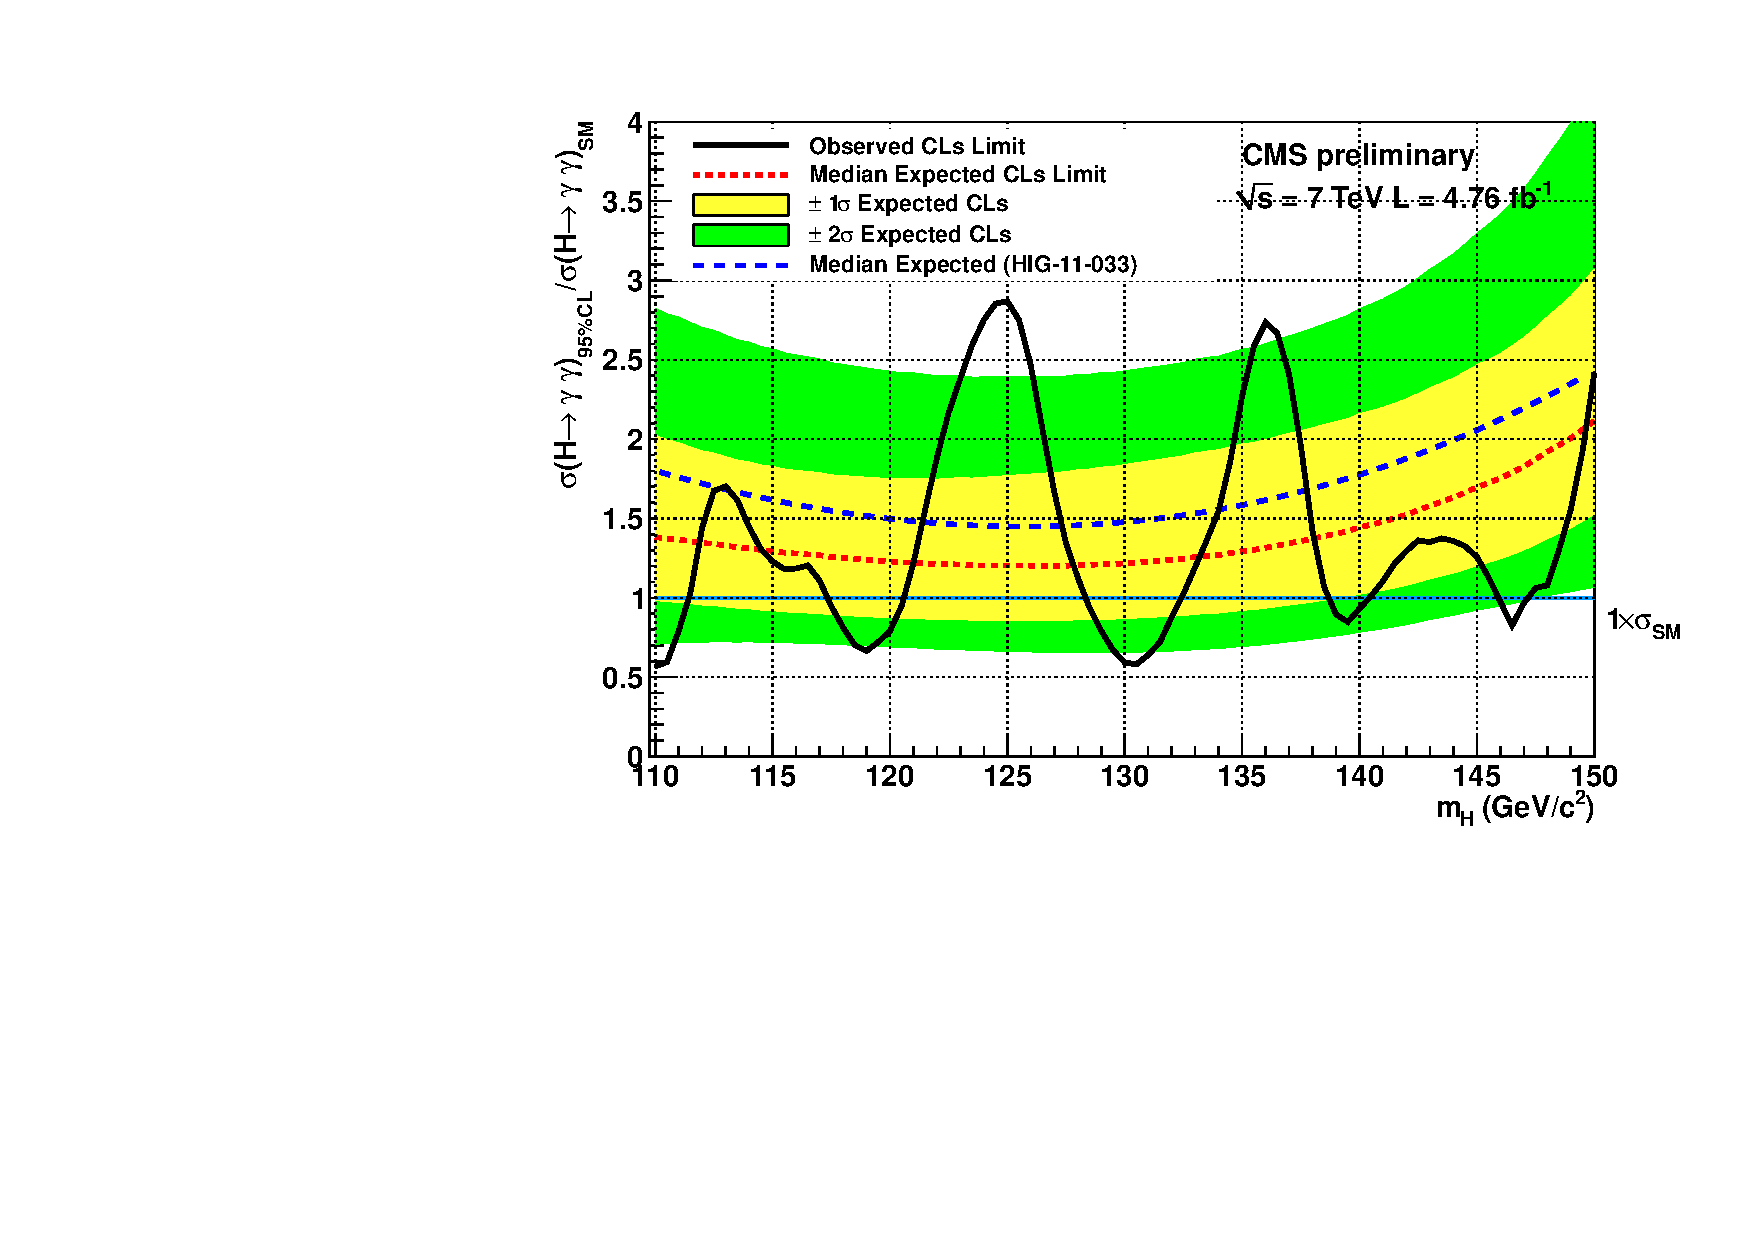
\includegraphics{LimitSMRelFreqCompare}}&
      \resizebox{6.5cm}{!}{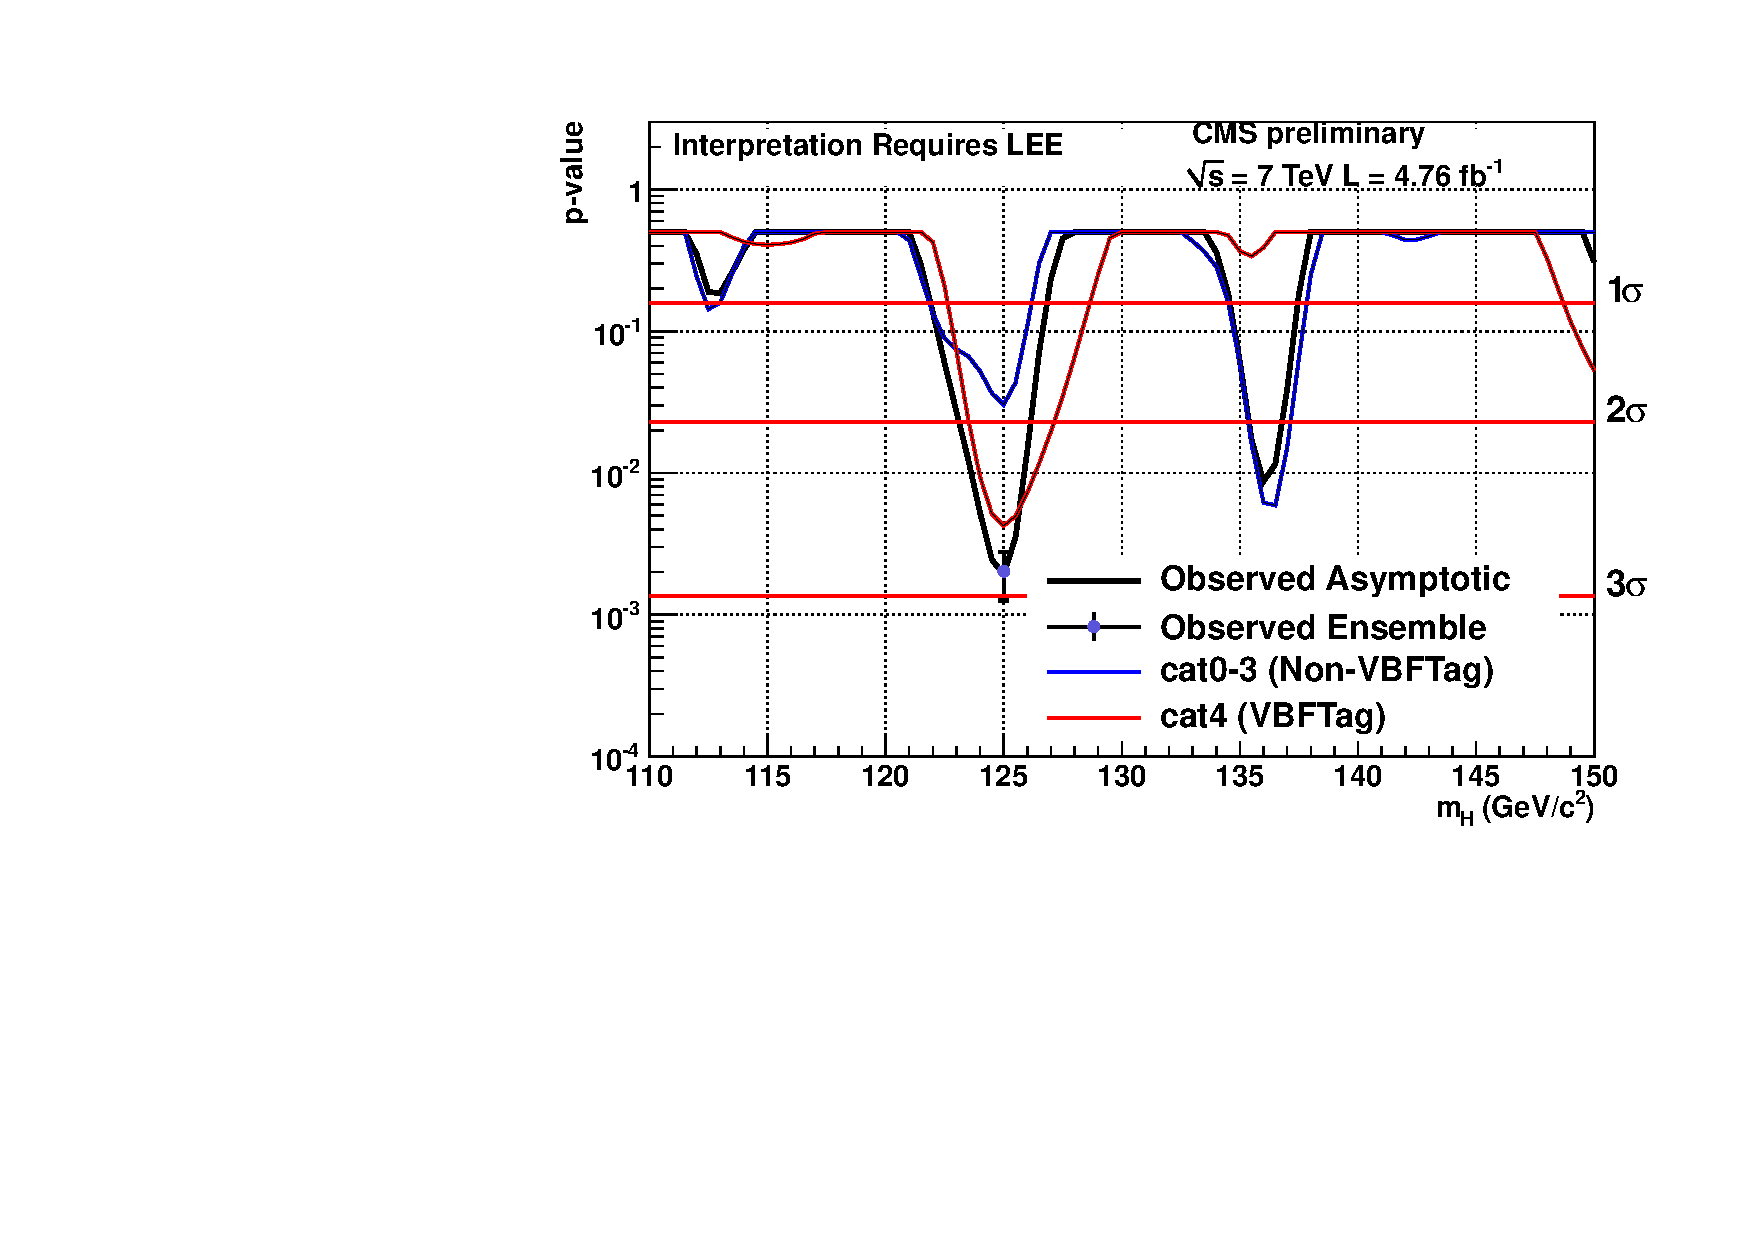
\includegraphics{pvaluesmcatc}}
    \end{tabular}
    \caption{Left: 95\% exclusion on the relative signal strength to
the SM in the $\gamma\gamma$ channel for the MVA based analysis. The
dashed line indicates the expected limit for the cut based
analysis. The yellow and green bands indicate the 1 and 2$\sigma$
expectations around the median expected result.  Right: local p-value
as function of the Higgs mass. The combined p-value is shown and the
VBF tag and other inclusive classes individual contributions are also
shown.  \label{fig:combpvaluegg}}
\end{center}
\end{figure} 







%%%%%%%%%%%%%%%%%
%
% Tau tau
% b bbar
%
%%%%%%%%%%%%%%%%%

\subsection{$H \to \tau\tau$ and $H \to bb$ channels}

These two channels are the only Higgs boson decays into fermions
detectable at LHC.  They are less sensitive than the
$H \to \gamma\gamma$ channel, but they would be important to measure
the couplings to leptons and quarks.
%% In both channels the background for the inclusive searches is huge
%% and sensitivity is improved by requesting additional tags such as
%% jets or charged leptons from VBF or VH production.
%
For the $\tau\tau$ channel the inclusive analysis is not very
sensitive, then we exploit the VBF topology as well as a boosted
topology. The mass reconstruction is not very precise due to the
presence of neutrinos in the decay and the resolution is approximately
20\%.  We search in the mass range between 110 and 150
GeV~\cite{Chatrchyan:2012vp}. The expected sensitivity for exclusion
is approximately 3 times the SM and we do not observe any significant
excess in the data~\cite{HIG-12-007,HIG-12-006}.
%
In case of the Higgs decays to bb, the background from bb, produced
via QCD, is much too large, so we need to exploit the VH associated
production with W and Z decaying leptonically and we analyze
separately all channels: $e\nu$, $\mu\nu$, ee, $\mu\mu$ and
$\nu\nu$~\cite{Chatrchyan:2012ww}.  We require the bb system to be
boosted to improve the background rejection and the mass resolution
that becomes about 10\%.  We search in the mass range between 110 and
135 GeV and the expected sensitivity for exclusion ranges from 3 to 6
times the SM.  Also in this channel we see no significant excess in
the data.



\section{Channels sensitive in the full mass range}

%%%%%%%%%%%%%%%%%
%
% WW
%
%%%%%%%%%%%%%%%%%

\subsection{$H \to WW \to 2\ell 2\nu$ channel}

This is the only viable channel for the Higgs boson search around the
mass region of $2\times\MW$ and the most sensitive in the mass range
of approximately 125--200 GeV.  The Higgs boson mass cannot be
precisely measured because of the undetected neutrinos and the
resolution is of the order of 20\%.  The signature is two isolated
high \pt leptons and the presence of missing transverse energy
(MET). 
The main backgrounds to this channel are WW production that is
irreducible, Z plus jets, WZ, ZZ and W plus jets. The main
backgrounds are estimated from the data.  A characteristic of the
signal is that due to the fact that the Higgs boson is a scalar and to
the V-A structure of the W decay, the two charged leptons tend to be
aligned. This favours a small difference in azimuthal angle
$\Delta\phi$ and provides some handle to discriminate the signal from
the irreducible background.  The analysis~\cite{Chatrchyan:2012ty} is
performed in exclusive jet multiplicities (0, 1 and 2-jet bins) and
flavour (ee, $\mu\mu$, e$\mu$) because of the different sensitivities
and background contributions. 
%% For example, the irreducible WW
%% background contributes more to the 0-jet bin, tt background
%% contributes more to the 1 and 2-jet bins and Z plus jets and ZZ
%% contribute more to same flavour analysis.  
The 2-jet bin corresponds to the VBF analysis and exploits the
characteristics of the VBF jets such as large \pt, large $\Delta\eta$
and di-jet invariant mass.  
%% Two types of analyses are carried out: the
%% first is a cut-and-count for all subchannels and the second is a
%% multivariate analysis that is applied to the 0 and 1-jet bins.
%% \begin{figure}[htbp]
%%   \begin{center}
%%       \resizebox{5.0cm}{!}{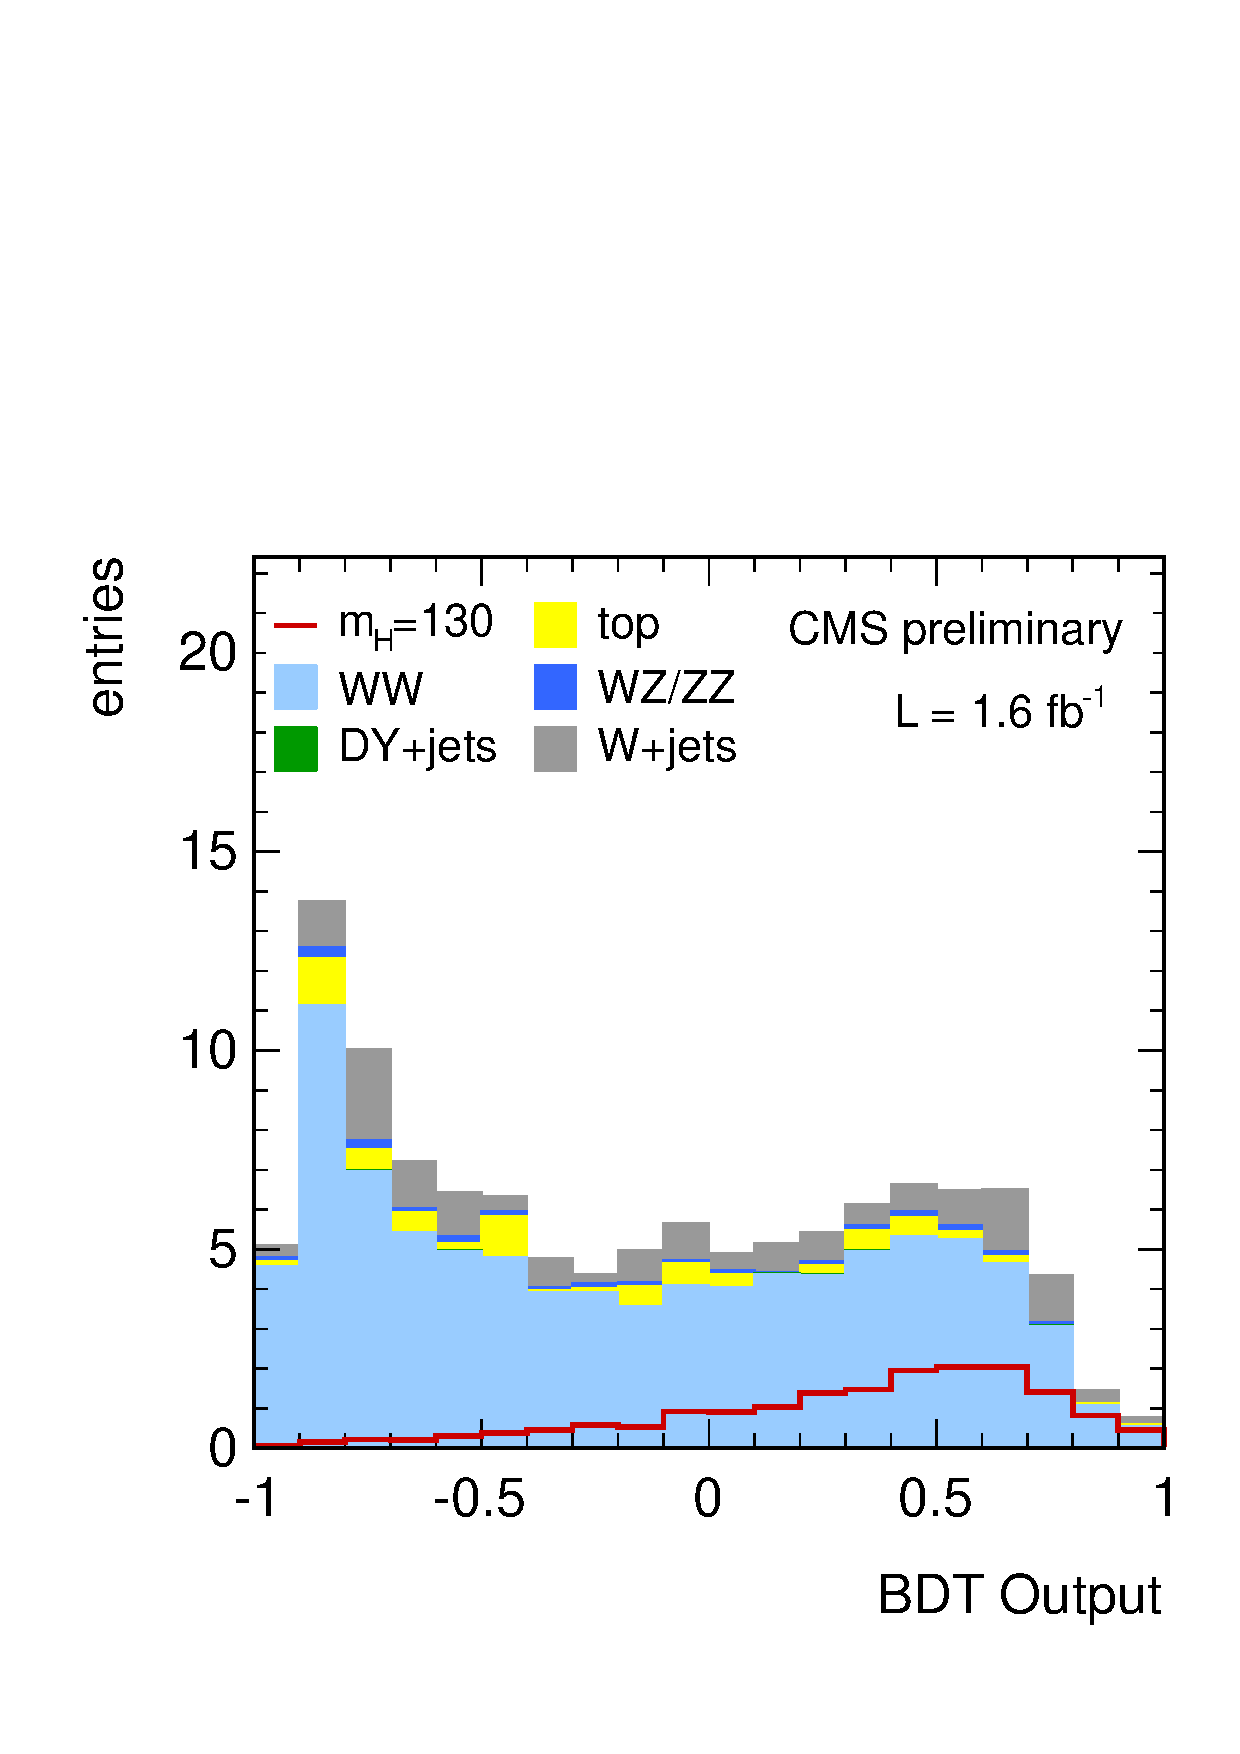
\includegraphics{histo_mva_130_0j_of}} 
%%       \resizebox{5.0cm}{!}{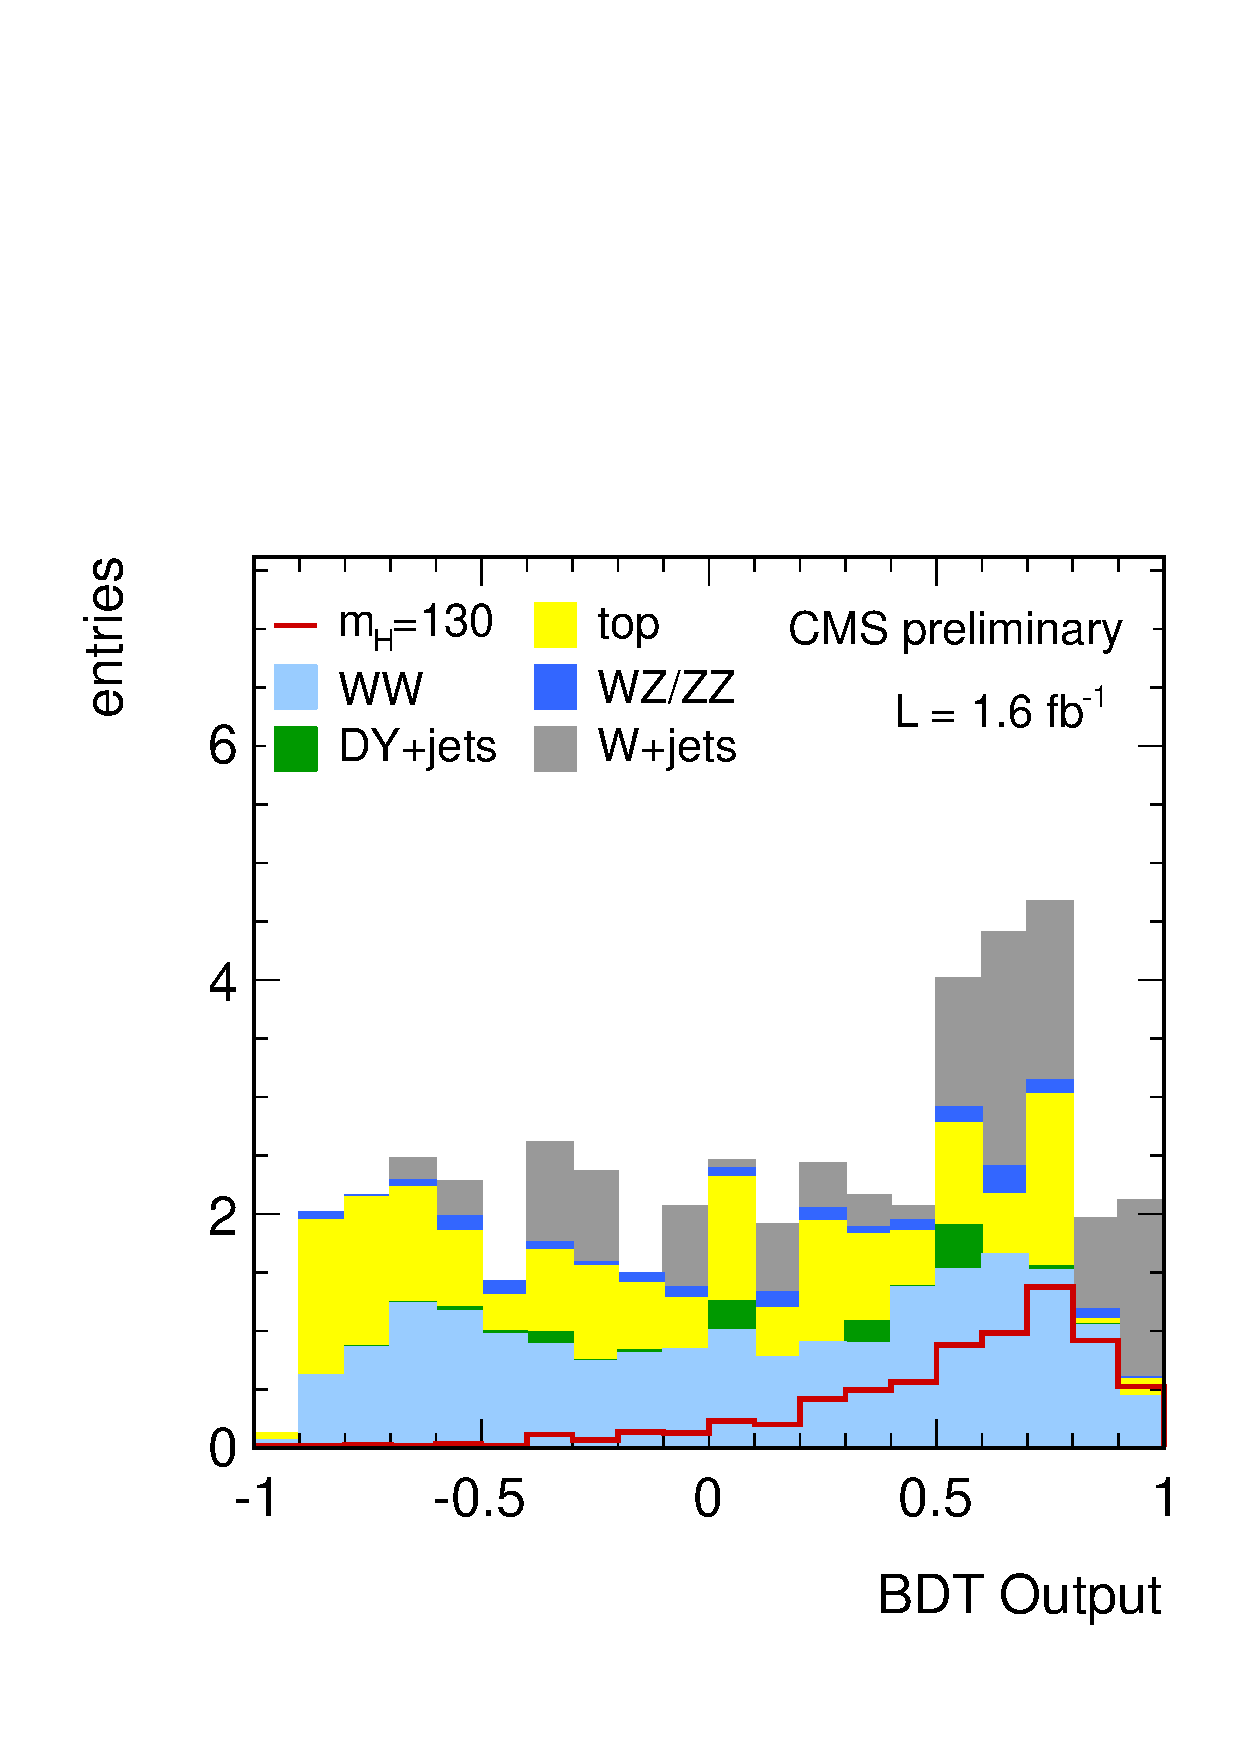
\includegraphics{histo_mva_130_1j_of}}
%%        \caption{BDT output for the 130 GeV $H \to WW \to
%%     2\ell 2\nu$ selection. Opposite flavour final state for 0-jet
%% (left) and 1-jet (right).  \label{fig:wwbdtdistrib}} 
%%    \end{center}
%% \end{figure} 
%% The MET is a very important variable in the analysis and is affected
%% by pileup, therefore it deserves a special treatment.  The so called
%% projected MET is used. It corresponds to the transverse component of
%% the MET with respect to the nearest lepton, if the angle between the
%% MET direction and the lepton is less than $\pi/2$, and to the full MET
%% otherwise.  Additionally, we compute two different flavours of MET:
%% the total MET using all reconstructed particles and the charged MET
%% using only the charged particles associated to the identified primary
%% vertex. The minimum between the two is used for the selection. This
%% procedure is found to reject better the background because the two
%% definition of MET are more correlated in case of genuine MET as it is
%% the case for the signal.  
Different cuts are applied in the different flavour and same flavour
channels. Cuts are tighter and a Z mass veto is applied in the same
flavour channels because they are more affected by the Drell Yan
background.  The cut based selection has mass dependent cuts while the
MVA based analysis uses a BDT trained at different masses.  
%% The input
%% variables are: \pt of the leptons, ${\mathrm M}_{\ell\ell}$,
%% $\Delta\phi_{\ell\ell}$, $\Delta\mathrm{R}_{\ell\ell}$, transverse
%% mass of the dilepton system and of each lepton and the MET.  
The overall uncertainties after the final selection are approximately 20\%
for the signal efficiency and 15\% for the expected background.  
%% The most sensitive channel is the opposite flavour 0-jet bin where the
%% signal is larger, the signal/background is larger and the background
%% is dominated by the irreducible WW that has less uncertainties than
%% the Z plus jets or tt contributions.
Figure~\ref{fig:WWlimit} shows the 95\% exclusion confidence level for
the cut based and the MVA shape analysis.  We observe no significant
excess in the full mass range though a small excess is observed at low
mass. Therefore the observed limits are similar to the expected ones.
For the MVA shape analysis the 95\% C.L. expected exclusion is
for \MH\ between 127 and 270 GeV and the range 129--270 GeV is
excluded at 95\% CL.
\begin{figure}[htbp]
  \begin{center}
    \begin{tabular}{cc}
      \resizebox{6.5cm}{!}{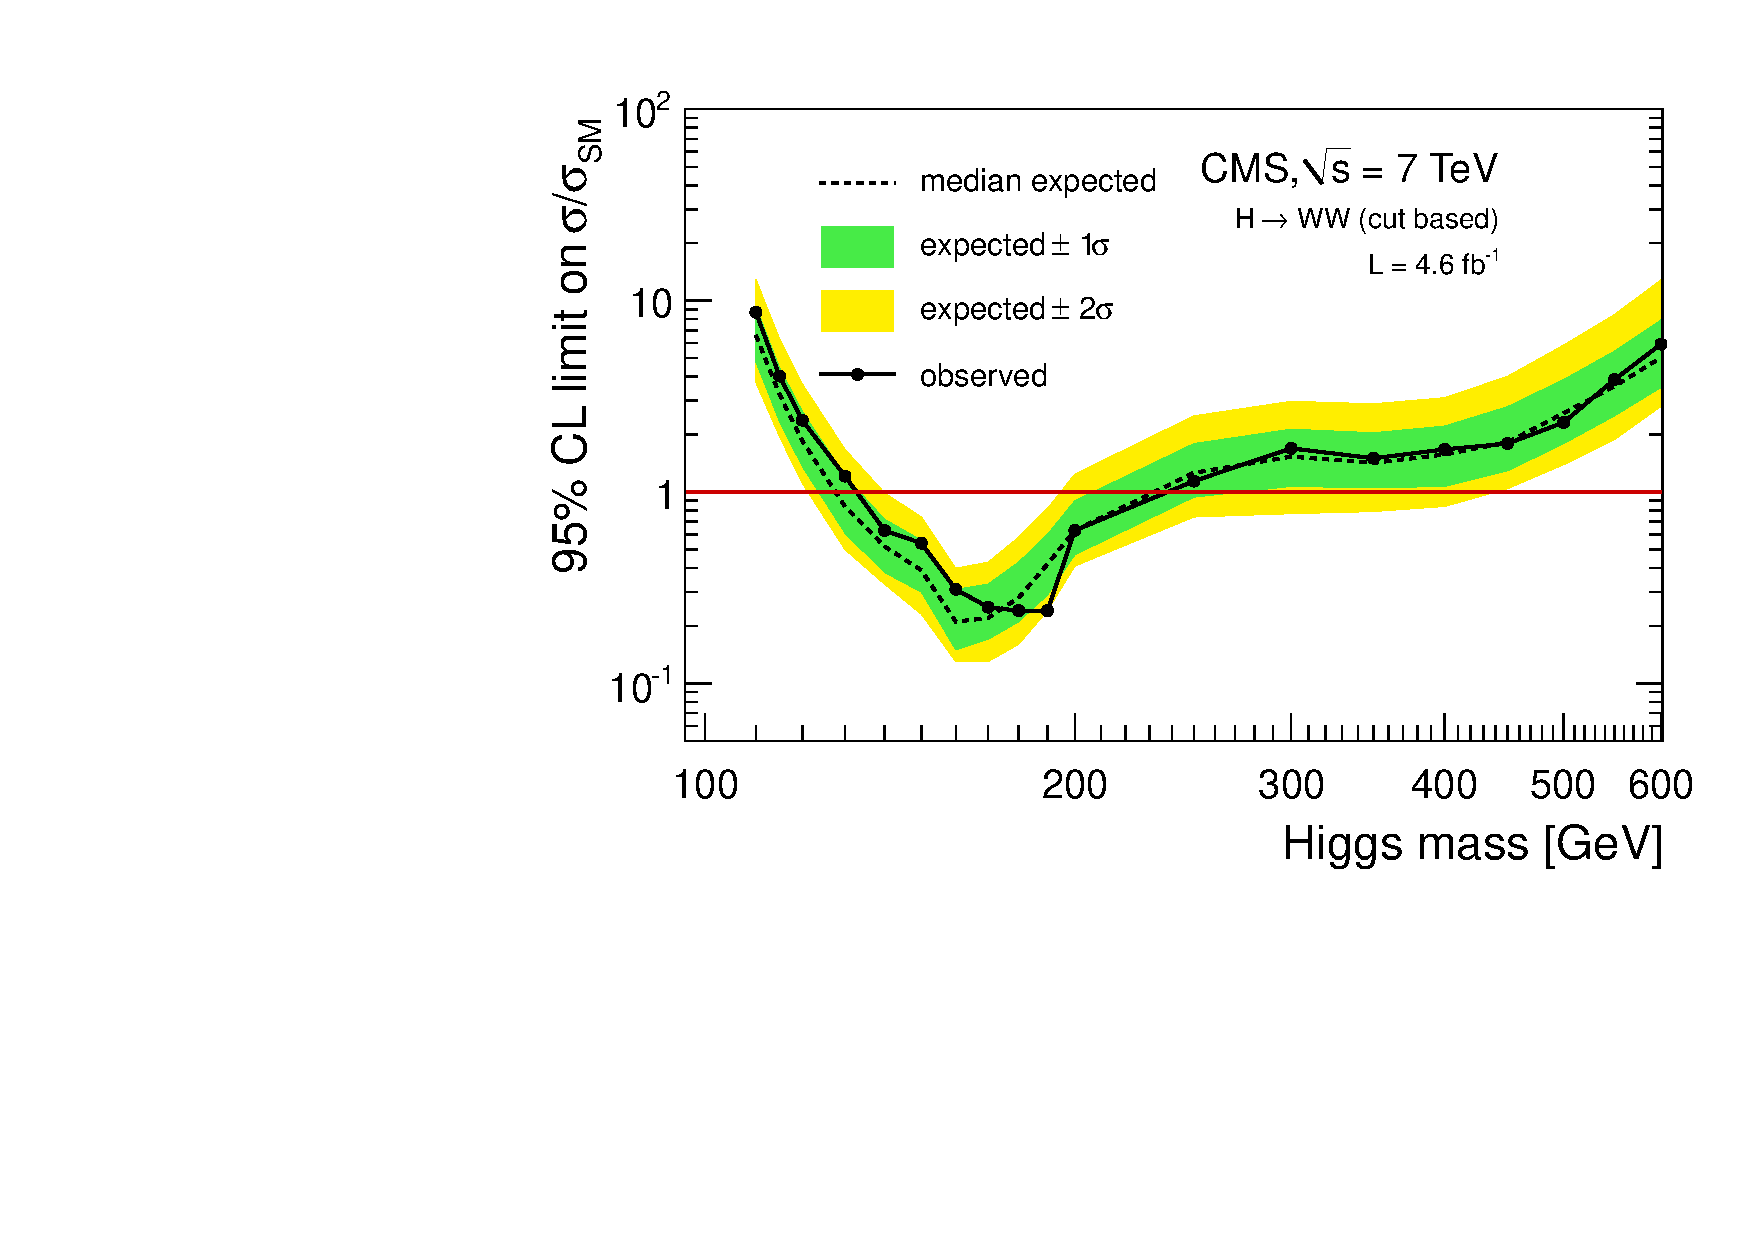
\includegraphics{limits_nj_cut}} &
      \resizebox{6.5cm}{!}{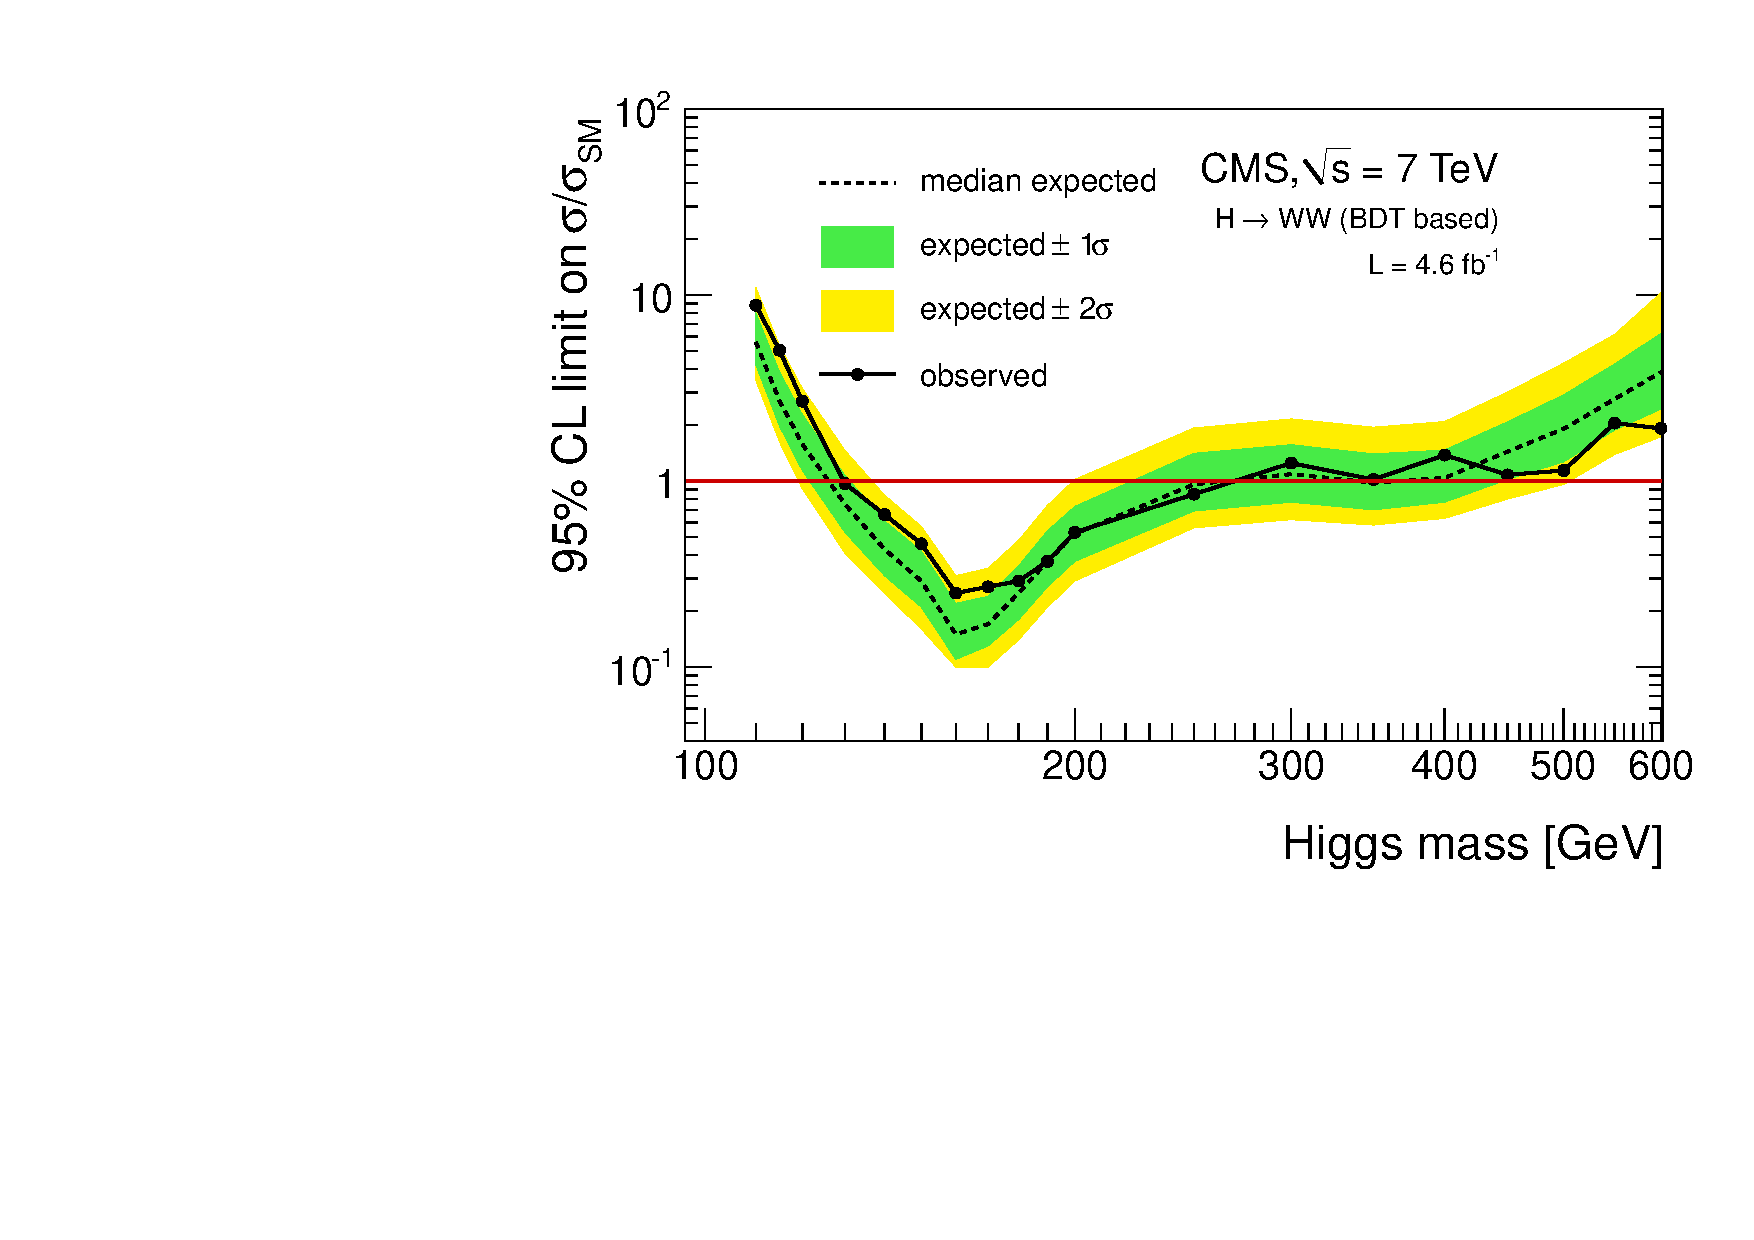
\includegraphics{limits_nj_shape}}
     \vspace*{-0.4cm}
    \end{tabular}
    \caption{95\% exclusion limit on the relative signal strength to the SM for the cut based analysis(left) and for the MVA analysis (right) in the $H \to WW \to 2\ell 2\nu$ channel.
    \label{fig:WWlimit}}
  \end{center}
\end{figure} 

%% \begin{table}[htbp]
%% %\color{black} 
%% \begin{center}
%% \caption{Expected background and observed data in the full mass range and in the mass range 100--160 GeV in the $H \to ZZ \to 4\ell$ channel.}
%% \begin{tabular}{|l|c|c|}
%% \hline
%% Mass range &  Expected background  & Observed data\\
%% \hline
%% Full mass range & $67\pm 6$ & 72\\
%% $M_{4\ell}$ in 100--160 GeV & $9.7\pm 1.3$ & 13\\
%% \hline
%% \end{tabular}
%% \label{tab:ZZevents}
%% \end{center} 
%% \end{table}




%%%%%%%%%%%%%%%%%
%
% ZZ
%
%%%%%%%%%%%%%%%%%
\subsection{$H \to ZZ \to 4\ell$ channel}

The $H \to ZZ \to 4\ell$ channel is the cleanest channel and it is
often referred as the ``golden channel''.  The signal consists of four
isolated leptons. For high mass both pairs of opposite charge and same
flavour leptons are consistent with Z decays while for lower masses at
least one of the pairs has lower mass.  The Higgs branching ratio for
this channel is rather small, approximately one per mille at high mass
and lower for masses below $2\times\MW$ but the background is very
small, consisting mainly of irreducible continuum ZZ production and,
to a lesser extent, Z plus jets and especially Zbb.  The mass
resolution is very good and ranges between 1 and 2\%.  The \pt of the
lower \pt leptons is rather small and one of the most important
features of the analysis is the achievement of a very high lepton
efficiency down to very low \pt.  The analysis is carried out in the
full mass range, from 110 to 600 GeV~\cite{Chatrchyan:2012dg}.

\begin{figure}[htbp]
  \begin{center}
    \begin{tabular}{cc}
      \vspace{-0.4cm}
      \resizebox{6.5cm}{!}{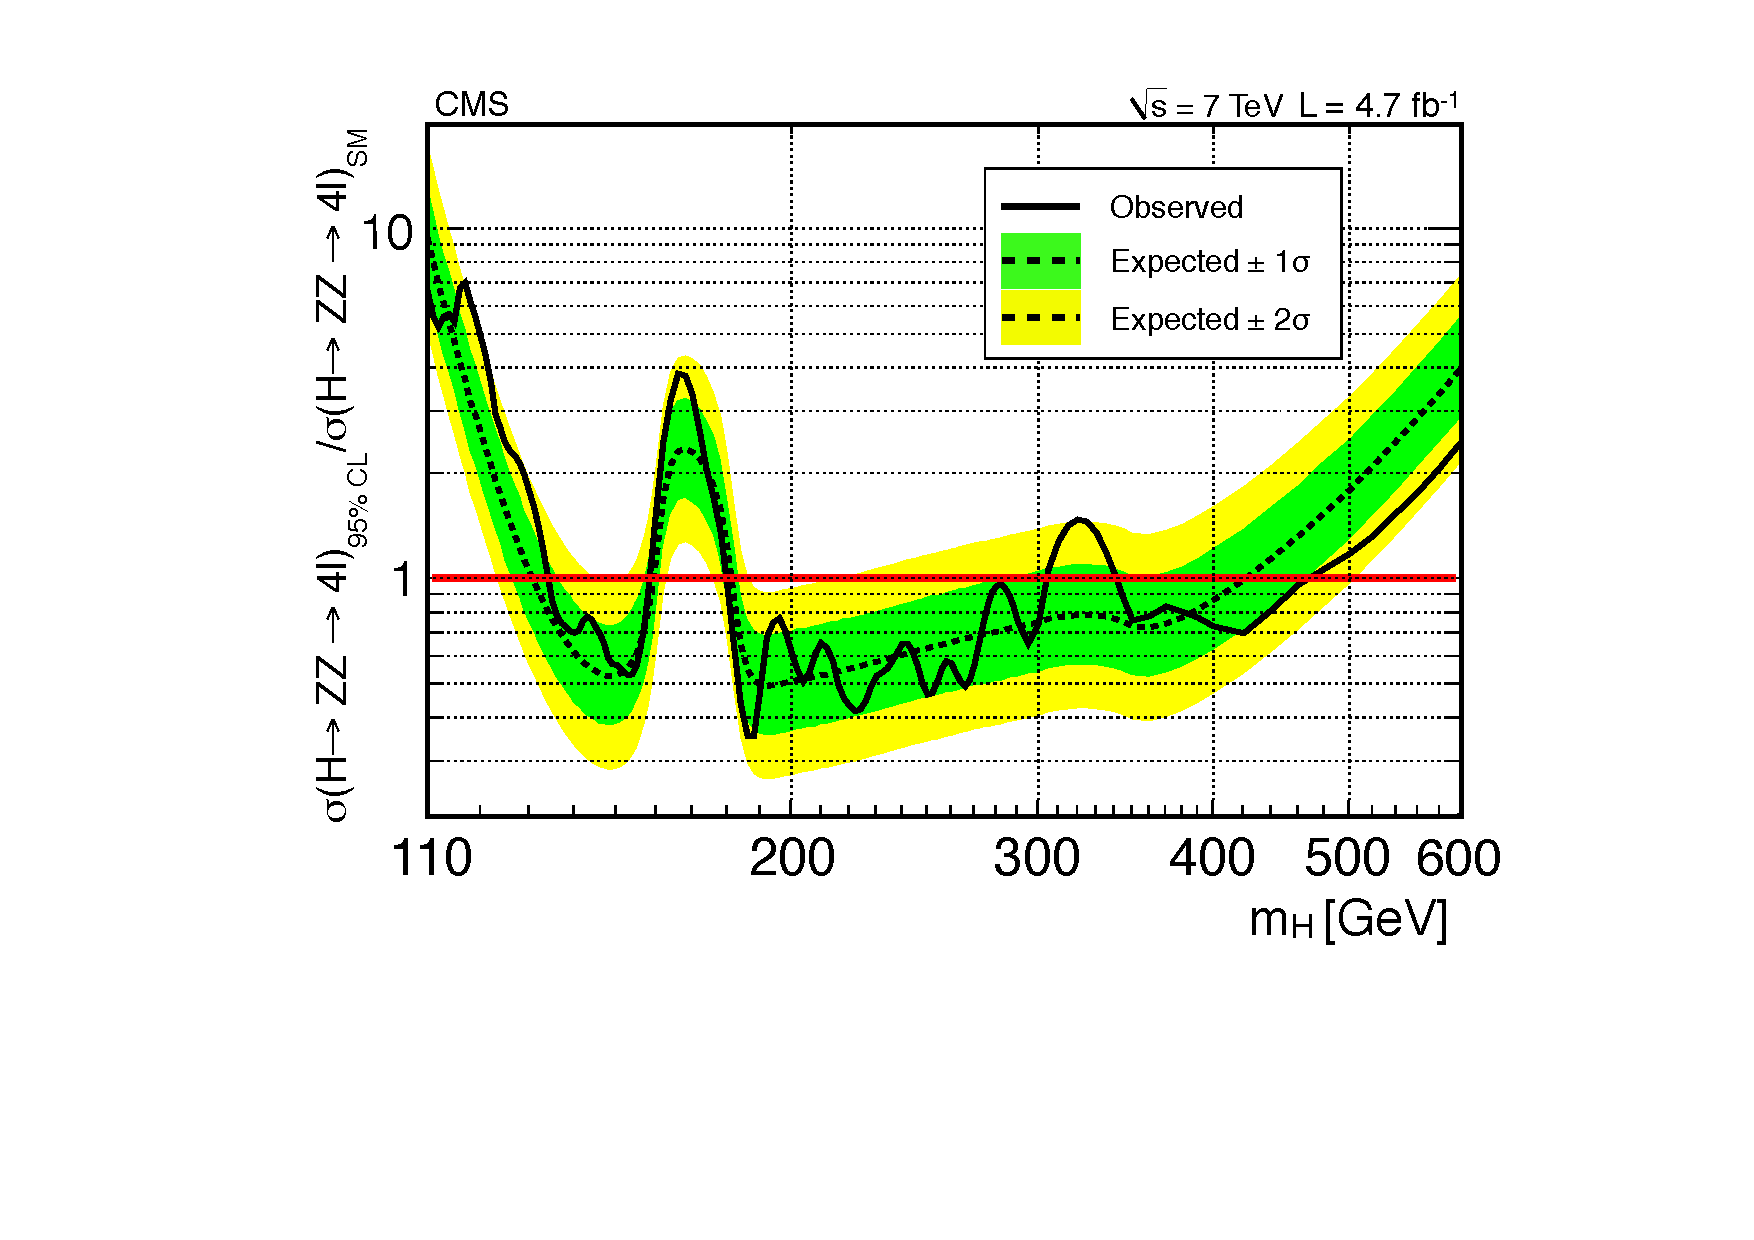
\includegraphics{UpperLimit_110_600_CLs}}
      &
      \resizebox{6.5cm}{!}{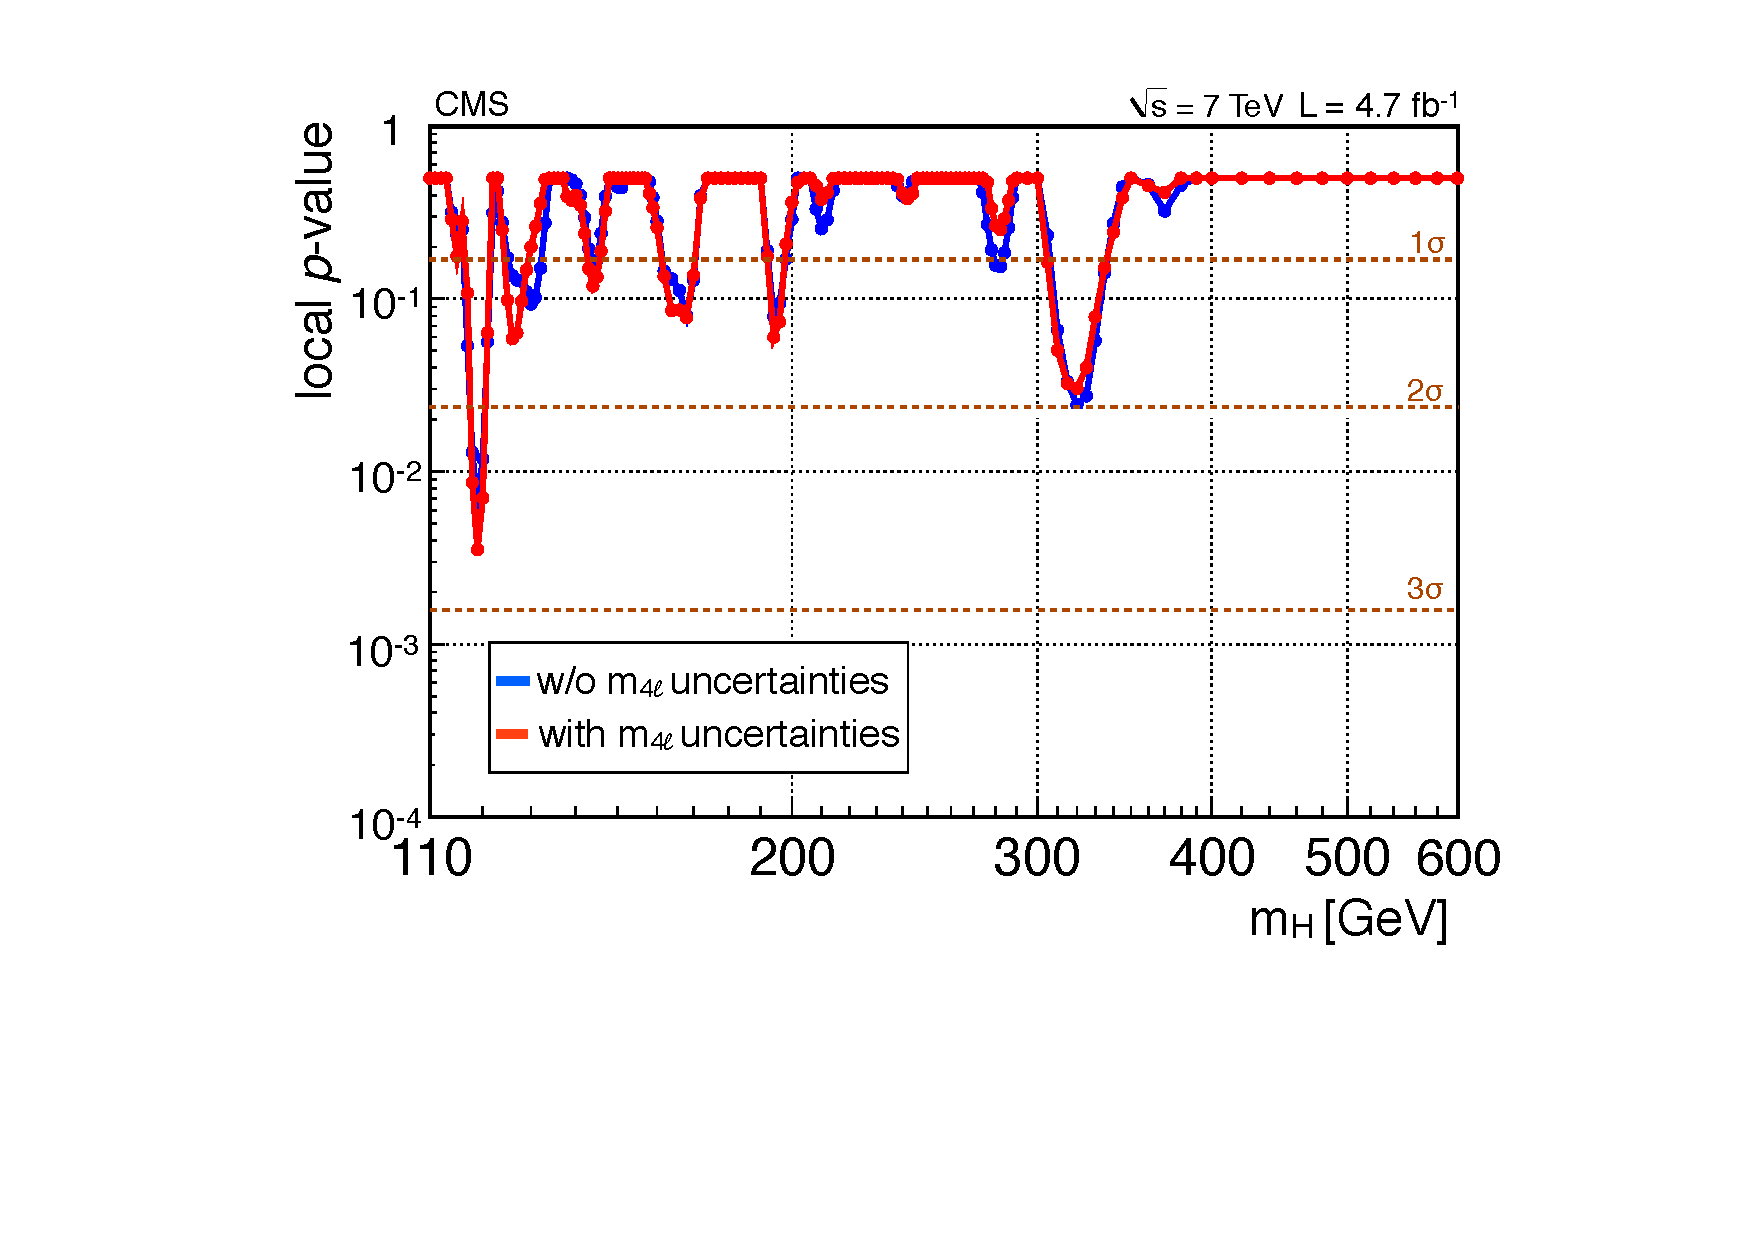
\includegraphics{pValue_110_600}}
    \end{tabular}

    \caption{95\% exclusion limit on the relative signal strength to the SM (left) and local p-value computed with and without the individual candidate errors on the reconstructed mass in the $H \to ZZ \to 4\ell$ channel.}
    \label{fig:ZZlimpvalue}
  \end{center}
      \vspace{-0.3cm}
\end{figure} 

We do not observe any significant excess of the data and we exclude at
95\% CL the SM Higgs boson with \MH\ in 134--158, 180--305 and
340--465 GeV.  The most significant excess is given by an accumulation
of 3 events at a mass of approximately 119.5 GeV.  It has a local
significance of 2.5$\sigma$ and a global significance of 1.0$\sigma$
in the full mass range and 1.6$\sigma$ in the mass range 100--160 GeV.






%%%%%%%%%%%%%%%%%%
%                %
%   HIGH MASS    %
%                %
%%%%%%%%%%%%%%%%%%


\section{High mass channels}

A SM Higgs boson above a mass of approximately 200 GeV almost
exclusively decays into WW and ZZ and above about 300 GeV the Higgs
boson width starts to be larger than the resolution in ZZ channels.
Beyond the previously described channels $H \to WW \to 2\ell 2\nu$ and
$H \to ZZ \to 4\ell$ channels, we searched in the channels where one Z
decays into $\nu$ ~\cite{Chatrchyan:2012ft},
quark~\cite{Chatrchyan:2012sn} and $\tau$ pairs
~\cite{Chatrchyan:2012hr}.  The first one has high sensitivity in
$\MH>250$ GeV, resulting in a 95\% CL exclusion of \MH\ in 270--440
GeV, the second has a little lower sensitivity, while the last has a
sensitivity of about 4 times the SM.

%% \subsection{$H \to ZZ \to \ell\ell\nu\nu$ channel}

%% The $H \to ZZ \to \ell\ell\nu\nu$ channel has a branching ratio 6
%% times larger that ZZ to $4\ell$ and is the most sensitive at very high
%% mass.  It is only accessible for high mass ($\MH>250$ GeV) because the
%% two Z bosons need to be boosted to give rise to MET by means of the Z
%% invisible decay.  Missing neutrinos worsen the mass resolution that is
%% about 7\% in this channel.  The main backgrounds in this channel are
%% again the irreducible ZZ process, Z plus jets, tt and WZ.  The main
%% backgrounds are estimated from data control samples.  Again in this
%% channel two independent analyses are carried
%% out~\cite{Chatrchyan:2012ft}: a cut based analysis and a mass shape
%% analysis, using transverse mass, that is more sensitive.  We did not
%% observe any excess in the data and the observed exclusion from this
%% channel alone is similar to the one expected in presence of background
%% only.  The expected 95\% CL exclusion using this channel alone is \MH\
%% in 290--480 GeV and the observed is \MH\ in 270--440 GeV.

%% \subsection{$H \to ZZ \to \ell\ell$qq and $H \to ZZ \to \ell\ell\tau\tau$ channels}

%% The $H \to ZZ \to \ell\ell$qq channel~\cite{Chatrchyan:2012sn} is used
%% both for the high mass, where its sensitivity is similar but a little
%% lower than the other ZZ channels, and for lower masses where it only
%% gives a small contribution to the sensitivity.  The $H \to
%% ZZ \to \ell\ell\tau\tau$ channel~\cite{Chatrchyan:2012hr} has a lower
%% sensitivity of about 4 times the SM.



\section{Combination of all channels and Summary}
\label{sec:Results}

All 11 searched channels using
approximately 5 \fbinv of 7 TeV pp collision data
are combined to obtain the final exclusion and
discovery confidence levels.  The combination is carried out using the
so-called CLs method described in~\cite{LHClimits}.  The present
combination that includes preliminary results is descibed
in~\cite{HIG-12-008}.  SM cross sections and branching ratios are
assumed for the combination with their theoretical
uncertainties~\cite{Dittmaier:2012vm}. An overall
signal strength multiplier $\mu=\sigma/\sigma_{\mathrm{SM}}$ is
introduced and limits on its value are derived.
%% Left figure~\ref{fig:combcl} shows the SM exclusion confidence level
%% as function of the Higgs boson mass.  
The SM Higgs boson is excluded
by our search at 95\% confidence level in the range 127.5--600 GeV and
at 99\% confidence level in the range 129--525 GeV.  The expected 95\%
exclusion is 114.5--543 GeV.  The observed CMS upper limit on the
Higgs boson mass is higher than expected in case of no signal because
of the excess that is observed in the data in the region between 115
and 128 GeV.
%% \begin{figure}[htbp]
%%   \begin{center}
%%     \begin{tabular}{cc}
%%       \resizebox{6.5cm}{!}{\includegraphics{sqr_smcls_comb_logx}}
%%       \resizebox{6.5cm}{!}{\includegraphics{pvala_all_zzc_t2_gz_zoom.png}} \\
%%     \end{tabular}

%%     \caption{Exclusion confidence level for the combined SM Higgs
%%     search in the full mass range 110--600 GeV (left) and combined
%%     local p-value for the SM Higgs search
%%     (right).  \label{fig:combcl}} 
%%    \end{center}
%% \end{figure} 
%% Right figure~\ref{fig:combcl} shows the local p-value as function of
%% the Higgs boson mass in the low mass region.  We can see that 
The minimum combined p-value is observed at a mass of 125 GeV with a local
significance of $2.8\sigma$.  A similar significance is expected in
presence of a 125 GeV Higgs boson signal.  
%% If we consider the
%% probability of observing a local significance smaller than $2.8\sigma$
%% anywhere in the search range, we obtain a global significance of
%% $0.8\sigma$ relative to the full mass range 110--600 GeV and of
%% $2.1\sigma$ for the mass range 110--145 GeV.
The fitted value of the signal strength multiplier
$\mu=\sigma/\sigma_{\mathrm{SM}}$ of the excess near 125 GeV is
consistent with the SM scalar boson expectation and several channels
show some excess, though most of it comes from the
$H \to \gamma\gamma$ channel.  The data that will be collected in 2012
at 8 TeV CM energy should allow us to discover or exclude the SM
scalar boson.

\section*{References}

\begin{thebibliography}{0}




\bibitem{SM1}{S.~Weinberg,} \textit{ Phys. Rev. Lett.} \textbf{ 19} (1967) 1264.
\bibitem{SM2}{A.~Salam, ``Elementary Particle Theory''}, p.~367.
\newblock Almquist and Wiksells, Stockholm, 1968.
\bibitem{Higgs1}{F. Englert and R. Brout}, \textit{ Phys. Rev. Lett.} \textbf{ 13} (1964) 321.
\bibitem{Higgs2}{P. W. Higgs}, \textit{ Phys. Rev. Lett.} \textbf{ 13} (1964) 508.
\bibitem{leplimits}{R.~Barate et al., \textit{ Phys. Lett.} \textbf{ B565} (2003) 61--75.}
\bibitem{tevatronlimits} {CDF and D0 Collaborations}, (July, 2011). {CDF Note 10606 and D0 Note 6226}.
\bibitem{Dittmaier:2012vm} S.~Dittmaier {\it et al.}, arXiv:1201.3084.
\bibitem{CMSdetector} CMS Collaboration, \textit{JINST} \textbf{3} (2008) S08004.
\bibitem{Chatrchyan:2012tw}  S.~Chatrchyan {\it et al.}  [CMS Collaboration], Phys.\ Lett.\  B {\bf 710}, 403 (2012)
\bibitem{HIG-12-001} CMS Collaboration, CMS Physics Analysis Summary CMS-PAS-HIG-12-001 (2012).
\bibitem{Chatrchyan:2012vp} S.~Chatrchyan {\it et al.}  [CMS Collaboration], arXiv:1202.4083 .
\bibitem{HIG-12-007} CMS Collaboration, CMS Physics Analysis Summary CMS-PAS-HIG-12-007 (2012).
\bibitem{HIG-12-006} CMS Collaboration, CMS Physics Analysis Summary CMS-PAS-HIG-12-006 (2012).
\bibitem{Chatrchyan:2012ww} S.~Chatrchyan {\it et al.}  [CMS Collaboration], Phys.\ Lett.\  B {\bf 710}, 284 (2012)
\bibitem{Chatrchyan:2012ty} S.~Chatrchyan {\it et al.}  [CMS Collaboration], Phys.\ Lett.\  B {\bf 710}, 91 (2012)
\bibitem{HIG-11-034} CMS Collaboration, CMS Physics Analysis Summary CMS-PAS-HIG-11-034 (2011).
\bibitem{Chatrchyan:2012dg} S.~Chatrchyan {\it et al.}  [CMS Collaboration], arXiv:1202.1997.
\bibitem{Chatrchyan:2012ft} S.~Chatrchyan {\it et al.}  [CMS Collaboration], JHEP {\bf 1203}, 040 (2012)
\bibitem{Chatrchyan:2012sn} S.~Chatrchyan {\it et al.}  [CMS Collaboration], arXiv:1202.1416 .
\bibitem{Chatrchyan:2012hr} S.~Chatrchyan {\it et al.}  [CMS Collaboration], JHEP {\bf 1203}, 081 (2012)
\bibitem{LHClimits} ATLAS and CMS Collaborations, ATLAS-CONF-2011-157, CMS HIG-11-023 (2011).
\bibitem{Chatrchyan:2012tx} S.~Chatrchyan {\it et al.}  [CMS Collaboration], Phys.\ Lett.\  B {\bf 710}, 26 (2012)
\bibitem{HIG-12-008} CMS Collaboration, CMS Physics Analysis Summary CMS-PAS-HIG-12-008 (2012).
\end{thebibliography}

\end{document}
\endinput
%%
%% End of file `cimsmple.tex'.
